\documentclass[12pt,a4paper,oneside]{article}
\usepackage[colorlinks=true,unicode]{hyperref}
\usepackage[utf8]{inputenc}
\usepackage[czech]{babel}
\usepackage{graphicx}
\usepackage{pdfpages}
\usepackage{listings}             % Include the listings-package
\textwidth 16cm \textheight 25cm
\topmargin -1.3cm 
\oddsidemargin 0cm
\usepackage{footnote}
\pagestyle{empty}
\begin{document}
\title{Testování modulu ALTIMET01A}
\author{Jakub Kákona, Eva Pomíchalová; kaklik@mlab.cz}
\maketitle

\thispagestyle{empty}
\begin{abstract}
Při realizaci projektu ABL01A bylo zjištěno, že snímání tlaku z čidla MPL3115A2 funguje navzdory specifikaci výrobce minimálně do výšky 16 km což je cca 10 kPa. Na druhou stranu interní tlakový atmosférický model je použitelný pouze do výšky cca 10 km ve větších výškách vykazuje značné nepřesnosti. Cílem tohoto dokumentu je popsat přesnější měření a kalibrace čidla v případě použití v barometrickém výškoměru pro balonovou sondu ABL01A
\end{abstract}

\begin{figure} [htbp]
\begin{center}
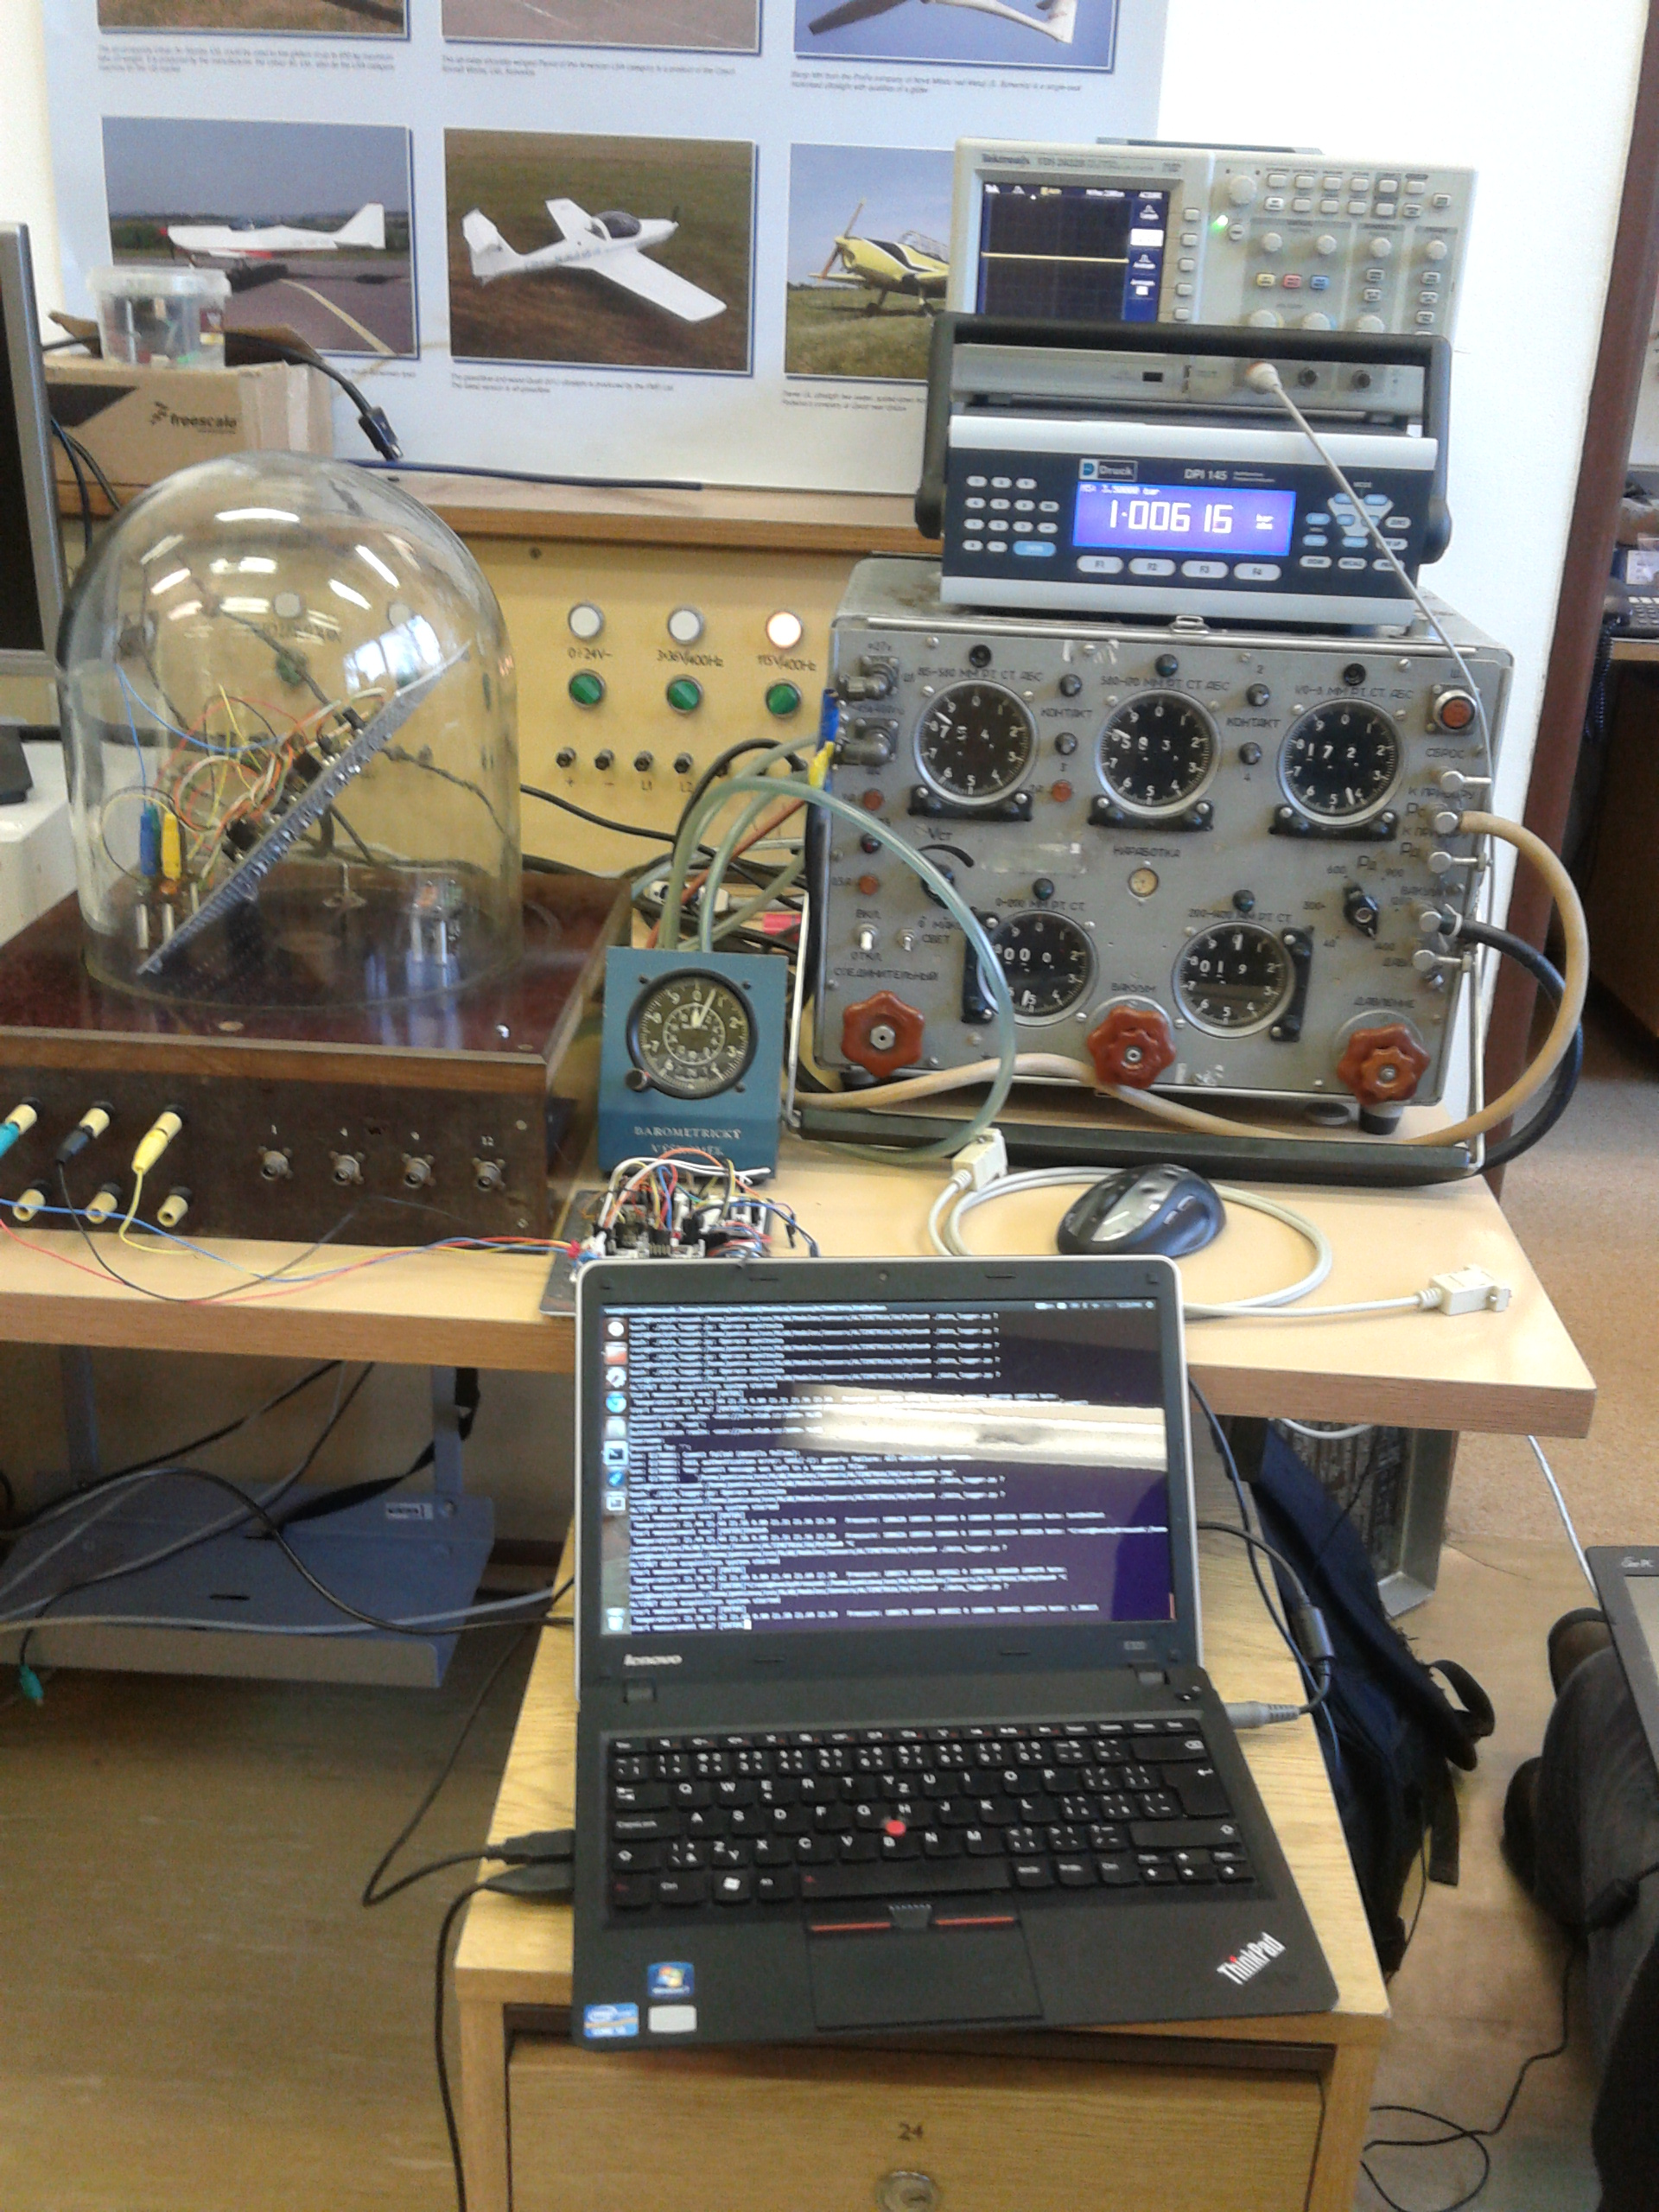
\includegraphics [width=80mm] {./img/altimet01a_testing_setup.jpg} 
\end{center}
\end{figure}

\begin{figure} [b]

\includegraphics [width=25mm] {./img/ALTIMET01A_QRcode.png} 
\end{figure}

\newpage
\tableofcontents
\newpage

\section{Popis konstrukce}

Realizace testovacího systému pro čidlo MPL3115A2 využívá modulu I2CHUB02A, který umožňuje testování více čidel najednou. Čidla jsou tak společně umístěna ve vakuovém zvonu s řízeným tlakem a naměřené tlaky jsou společně s teplotami vyčítány I$^2$C sběrnici. Sběrnice I$^2$C byla z řídícího počítače vyvedena přes převodník USB-AVR-i2c. 
Paralelně k hodnotám získaných z modulů ALTIMET je z řídícího počítače ještě vyčítán tlak měřený z referenčního měřícího přístroje DPI 145. 

Měřící přístroj DPI 145 byl do systému zapojen přes rozhraní RS232 za použití převodníku  RS232-USB. Nastavení komunikace je Parity=none, Speed=9600, Handshaking=none. (Způsob nastavení je možné nalézt v návodu k DPI145). 

\section{Programové vybavení}

Pro vyčítání čidel a záznam naměřených hodnot byl použit Python. Využívající speciálně vytvořenou knihovnu  \cite{MLAB-I2c-modules}. Tato knihovna řeší komunikaci se senzory MPL3115A2 v modulech ALTIMET01A. Samotný program je pak umístěn v dokumentační složce modulu ALTIMET01A \cite{data_logger}.

Na začánku programu je nadefinována topologie zapojení modulů, což je viditelné v následujícím bloku kódu (Odsazení bylo upraveno za účelem vložení na šířku stránky).

\lstset{language=Python}
\begin{lstlisting}[frame=single]
cfg = config.Config(
    port = port,
    bus = [
        {
            "type": "i2chub",
            "address": 0x72,
            
            "children": [
                {
                    "type": "i2chub",
                    "address": 0x70,
                    "channel": 3,
                    "children": [
{"name": "altimet1", "type": "altimet01" , "channel": 0, },   
{"name": "altimet2", "type": "altimet01" , "channel": 3, },   
{"name": "altimet3", "type": "altimet01" , "channel": 4, },   
{"name": "altimet4", "type": "altimet01" , "channel": 5, },   
{"name": "altimet5", "type": "altimet01" , "channel": 6, },   
{"name": "altimet6", "type": "altimet01" , "channel": 7, },   
                    ], 
                },
{"name": "altimet8", "type": "altimet01" , "channel": 6, },
            ],
        },
    ],
)
cfg.initialize()
\end{lstlisting}

Grafickou realizaci této topologie představuje obrázek \ref{test_setup_blocks}. V kterém jsou vynechána čísla portů na modulu I2CHUB02A. Podle nich jsou ve skutečnosti identifikována jednotlivá čidla, která jinak mají stejnou I2C adresu. Na sběrném počítači byl použit operační systém Linux Ubuntu 13.10.

\begin{figure} [htbp]
\centering
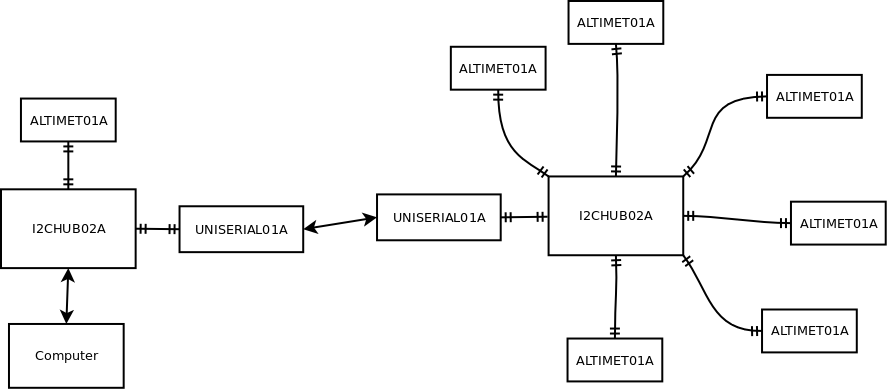
\includegraphics [width=220mm, angle=90, origin=c] {./img/test_setup.png}
\caption{Zapojení jednotlivých modulů v testovacím přípravku.}
\label{test_setup_blocks}
\end{figure}

\subsection{Čtení dat z přístroje DPI145}

Vzhledem k tomu, že přístroj byl připojený přes rozhraní RS232 a ke komunikaci používá protokol SCPI, tak bylo možné jej ovládat přímo z jazyka Python zápisem na seriové rozhraní počítače. V následujícím bloku je uveden testovací kód, který vyčte data zobrazena na displeji (Měřící přístroj musí být nastaven tak, aby na displeji byla přímo hodnota, kterou potřebujeme zaznamenat).

\begin{lstlisting}[frame=single]
#!/usr/bin/python

# Druck DPI 145  preassure measuring instrument test utility.  

import serial

ser = serial.Serial('/dev/ttyUSB0', 9600, timeout=1)
print ser.name
ser.write(':DISP?\n')
P_ref = eval(ser.readline(100))
sys.stdout.write("%s",P_ref)
ser.close()
\end{lstlisting}

Data jsou přijata ve formě stringu. Pro získání numerické proměnné by bylo třeba je parserovat  a vyhledávat číselný obsah. 

\section{Výsledky}

\subsection{Systém sběru dat z tlakových čidel}

Pro testování modulu ALTIMET01A s tlakovým čidlem MPL3115A2 byl vytvořen testovací přípravek využívající I2C a převodník USB-avr-i2c. Měřící systém byl ovládán skriptem napsaným v jazyce Python spouštěném na linuxovém počítači.  

\begin{thebibliography}{99}
\bibitem{MLAB-I2c-modules}{https://github.com/MLAB-project/MLAB-I2c-modules} 
\href{https://github.com/MLAB-project/MLAB-I2c-modules}{MLAB-I2c-modules}
\bibitem{data_logger}{svn://svn.mlab.cz/mlab/Modules/Sensors/ALTIMET01A/SW/Python} 
\href{svn://svn.mlab.cz/mlab/Modules/Sensors/ALTIMET01A/SW/Python}{MLAB-I2c-modules}
\end{thebibliography}
\end{document}